\chapter{Progettazione}

In questo capitolo viene descritta l'architettura del progetto, derivata dall'analisi dei requisiti.

\section{Architettura del sistema}
Il sistema è costituito da due macro parti:
\begin{itemize}
 \item un server che costituisce il punto di centralizzazione;
 \item un insieme di dispositivi embedded che dialogano con il server.
\end{itemize}
I dispositivi embedded hanno un comportamento locale, ovvero gestito individualmente da ognuno, e uno globale, cioè che richiede interazioni con il server centrale. Quest'ultima parte costituisce l'elemento di maggiore criticità, in quanto la quasi totalità delle interazioni si concentra sul server. Per far fronte ai requisiti di performance, reattività, scalabilità, facilità di gestione e interoperabilità, si è scelto di adottare REST come strategia di comunicazione, poiché possiede le seguenti caratteristiche fondamentali:
\begin{itemize}
 \item la comunicazione è di tipo client-server come richiesto;
 \item la comunicazione è ``stateless'', ovvero non necessita della memorizzazione di alcun contesto client sul server;
 \item consente di implementare facilmente un'architettura scalabile a livelli con nodi di commutazione intermedi;
 \item è universalmente riconosciuta e supportata, basandosi su HTTP + TCP + IP.
\end{itemize}
\subsection{Nota sull'utilizzo dei Raspberry PI}
Nella realizzazione di questo progetto si è scelto di utilizzare dispositivi Raspberry PI come dispositivi embedded, in quanto largamente noti e utilizzati. Da qui in avanti si parlerà di Raspberry, tuttavia anche altre tipologie di sistemi embedded possono essere utilizzate senza problemi, compresi microcontrollori. In questo modo si potrebbero ridurre i costi.


\section{Progettazione Server}
Il server (o il cluster di server, a seconda dell'implementazione) deve fornire i seguenti servizi:
\begin{itemize}
 \item un server web che fornirà un'interfaccia centralizzata per l'invio di comandi ai Raspberry;
 \item una servlet che si occuperà di ricevere attraverso un'interfaccia REST messaggi provenienti dai Raspberry, che funge da intermediaria tra i Raspberry e i database;
 \item un Time Series DBMS sul quale sono registrati i cambiamenti di stato segnalati dalla servlet;
 \item un sistema di generazione di statistiche e grafici basati sui dati contenuti nel Time Series DBMS;
 \item un DBMS relazionale per l'archiviazione di credenziali d'accesso e indice dei Raspberry che fanno parte del sistema;
\end{itemize}

\subsection{Tipologia del server}
Poiché la parte server ricopre un ruolo centrale nel sistema, è necessario valutare le alternative a disposizione, per poi scegliere quella più idonea:
\begin{itemize}
 \item acquisto di server dedicati;
 \item server cloud di tipo ``Infrastructure as a Service'' (IaaS);
 \item server cloud di tipo ``Platform as a Service'' (PaaS).
\end{itemize}
\paragraph{Acquisto di server dedicati}
Una prima possibilità è quella di acquistare server dedicati. Questa modalità prevede un investimento iniziale maggiore e richiede di gestire direttamente tutti i costi di gestione nel tempo, quali elettricità, sistemi di raffreddamento, gruppi di continuità, sostituzione dei componenti difettosi, impiego di personale specializzato. Questo potrebbe essere un problema nel caso i server da gestire (compresi anche quelli non collegati a questo sistema) fossero pochi, in quanto i costi difficilmente sarebbero ammortizzati. Ma soprattutto, le necessità in termini di prestazioni in un sistema di questo tipo possono essere molto variabili con il crescere del sistema stesso. Una città che optasse per l'acquisto di server dedicati, dovrebbe necessariamente acquistarli con prestazioni sovradimensionate rispetto all'utilizzo iniziale, in previsione dell'utilizzo a regime.
\paragraph{Server cloud IaaS}
Una seconda possibilità è quella di affidarsi ad un provider di servizi cloud ``IaaS'', che consentirebbe allo stesso tempo di spostare i costi di gestione e manutenzione del server all'interno di un datacenter. Sarebbe comunque necessario un sistemista per l'installazione e la manutenzione regolare del software del server, a partire dal sistema operativo. Inoltre, diventa possibile un rapido ridimensionamento delle risorse hardware allocate ai server, per far fronte alle richieste crescenti nel tempo (ipotizzando che i Raspberry vengano installati in maniera progressiva), riducendo i costi iniziali.
\paragraph{Server Cloud PaaS}
Utilizzando server cloud ``PaaS'', l'astrazione si sposta di un livello verso l'alto, in quando si rimuove la necessità di gestire il sistema operativo, focalizzandosi solo sui servizi. In questo modo si semplifica ulteriormente la gestione, a costo di una minore configurabilità dei servizi (si è molto più soggetti all'offerta del provider scelto).
\paragraph{Scelta finale}
Valutate le alternative, si è deciso di scartare l'acquisto di server dedicati, poiché si è ritenuto importante consentire il rapido ridimensionamento delle risorse hardware dedicate, garantendo scalabilità. Tra le due soluzioni ``IaaS'' e ``PaaS'' si è scelta la prima, in quanto le attuali proposte ``Paas'' sul mercato sono state ritenute troppo limitanti nelle funzionalità per il tipo di sistema che si vuole realizzare.

\subsection{Server Web}
TODO
%\begin{figure}[ht] % Nota: immagine già messa sotto nel rasp
%	\centering
%	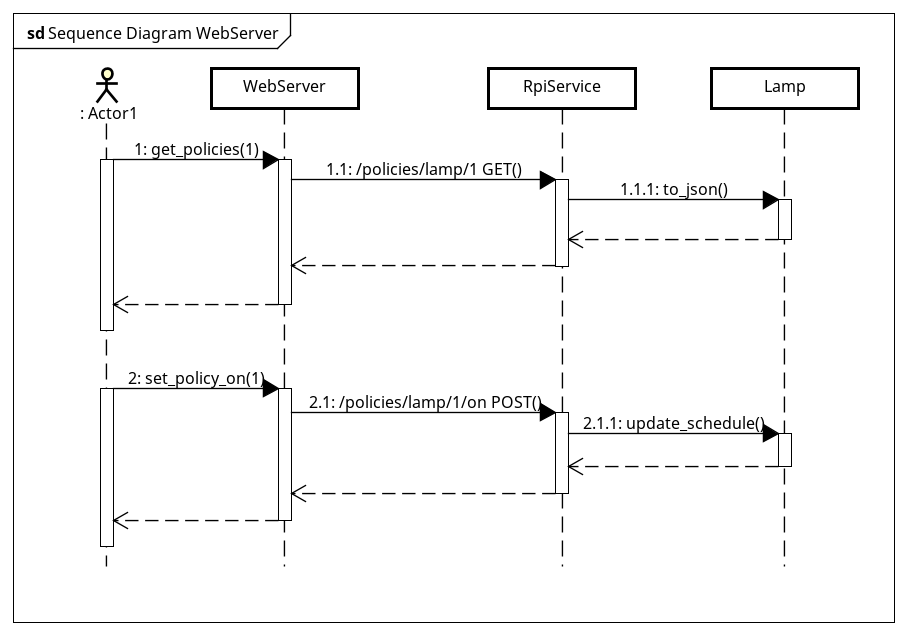
\includegraphics[scale=.8]{figure/Sequence_Diagram_WebServer.png}
%	\caption{Diagramma di sequenza delle comunicazioni tra  \label{FSM POLICY}}
%\end{figure}
\subsection{Servlet}
TODO
\iffalse
\begin{figure}[ht]
	\centering
	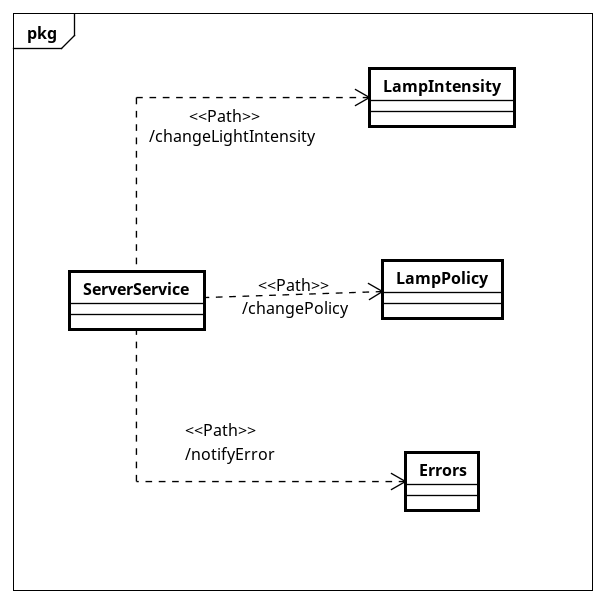
\includegraphics[scale=.8]{figure/Class_Diagram_Server_REST.png}
	\caption{API REST Servlet \label{API REST SERVLET}}
\end{figure}
\begin{figure}[ht]
	\centering
	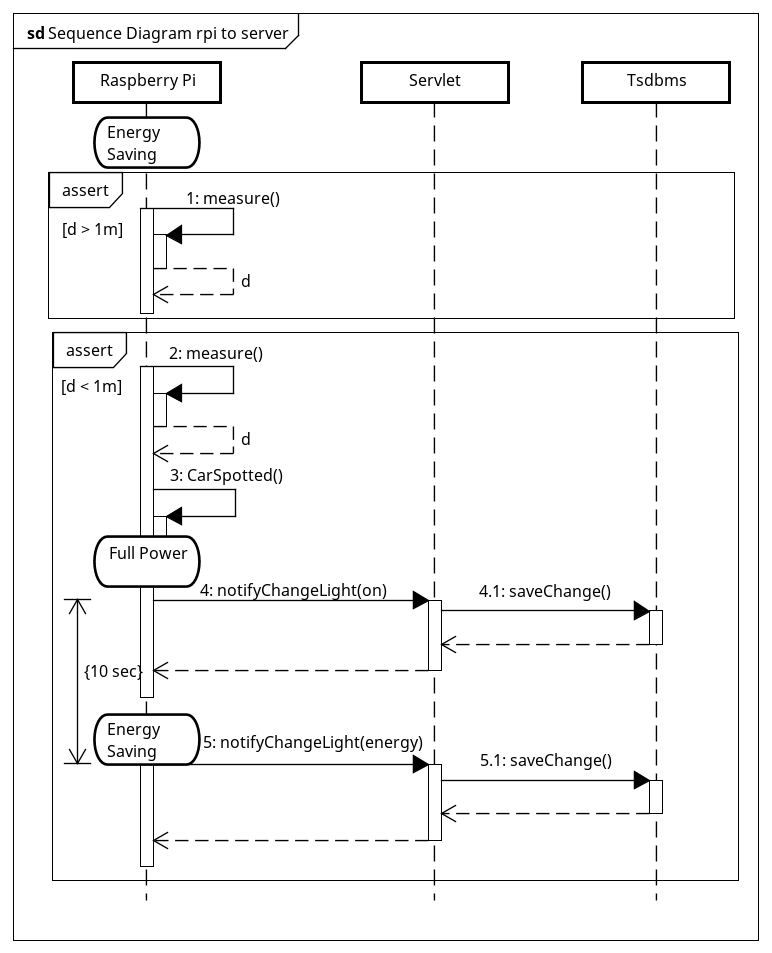
\includegraphics[scale=.8]{figure/Sequence_Diagram_rpi_to_server.png}
	\caption{Diagramma di sequenza delle comunicazioni tra Raspberry, servlet e TSDBMS \label{SEQ RPI TO SERVER}}
\end{figure}
\fi
\subsection{Time Series DBMS}
TODO
\subsection{Sistema di generazione di statistiche e grafici}
TODO
\subsection{DBMS relazionale}
TODO


\section{Progettazione Raspberry}
Il sistema Raspberry fornisce le seguenti funzionalità:
\begin{itemize}
 \item rilevamento illuminazione ambientale con il sensore di luce;
 \item rilevamento presenza di automobili con i sensori di prossimità;
 \item illuminazione di ogni singolo lampione in base alle politiche locali;
 \item programma principale che gestisce il web server REST e l'invio delle statistiche al server.
\end{itemize}

\subsection{Architettura complessiva}
yes
TODO class diagram Raspberry Pi

\subsection{Raspberry Pi architettura REST}
TODO

\subsection{Policy del sistema}
L'eventuale illuminazione di un lampione è regolata da policy decise a priori e modificabili anche durante l'esecuzione del sistema.
A meno della rilevazione del passaggio di un'auto o di un livello di intensità luminosa eccedente il limite impostato nelle policy, l'unico fattore che viene usato per l'illuminazione è l'orario corrente.
\paragraph{Macchina a stati finiti}
Per mostrare il comportamento del sistema riguardante le policy temporali si è utilizzata la macchina a stati finiti semplificata di figura \ref{FSM POLICY}.
Inizialmente i lampioni partono dallo stato "off" e se l'orario corrente (rappresentato dalla variabile t) è successivo all'orario impostato per la policy on, allora il lampione passerà allo stato "on". In seguito quando l'orario supererà la soglia di policy energy on, il lampione andrà in modalità risparmio energetico passando allo stato "energy saving".
Alla fine del periodo di risparmio energetico, impostato da policy energy off, il lampione tornerà allo stato di partenza spegnendosi.
\begin{figure}[ht]
	\centering
	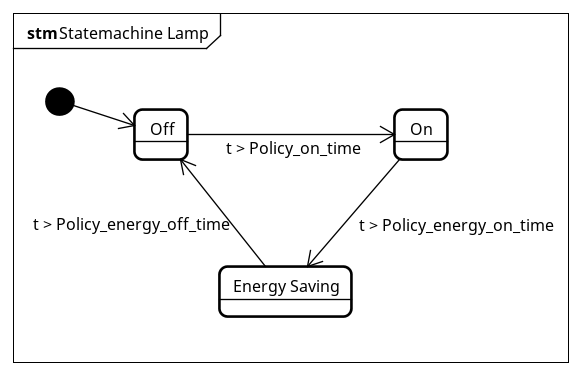
\includegraphics[scale=.8]{figure/Statemachine_Lamp.png}
	\caption{Finished State Machine relativo alle policy del sistema \label{FSM POLICY}}
\end{figure}

\newpage
\subsection{Controllo presenza auto}
Questa parte si occupa di controllare la presenza di eventuali auto in transito. Utilizzando un sensore di prossimità periodicamente viene calcolata la distanza tra il sensore e l'ostacolo più vicino per valutare se un'auto possa essere in transito in quel momento sulla carreggiata.
\paragraph{Comportamento sensore di prossimità}
Per la rappresentazione dell'architettura è stato scelto di utilizzare una Finished State Machine.
Come si può notare in figura \ref{FSM CAR} all'avvio dell'ultrasonic vengono creati due thread concorrenti. Il primo ha il compito di aggiungere e rimuovere i lampioni interessati ad essere notificati del passaggio di auto.
Il secondo invece si occupa di fare la rilevazione della distanza tra il sensore e l'oggetto in quel momento più vicino. Partendo dallo stato "waiting", se è presente almeno un attore, viene effettuata una lettura di distanza e, se il valore è maggiore di 1 metro, aspetta 200 millisecondi per poi tornare nello stato "waiting". Se invece il valore è minore di 1 metro significa che è stata rilevata un auto e quindi vengono notificati tutti i lampioni attualmente in lista. Dopo aver aspettato 5 secondi torna allo stato iniziale di "waiting".
\begin{figure}[tbp]
	\centering
	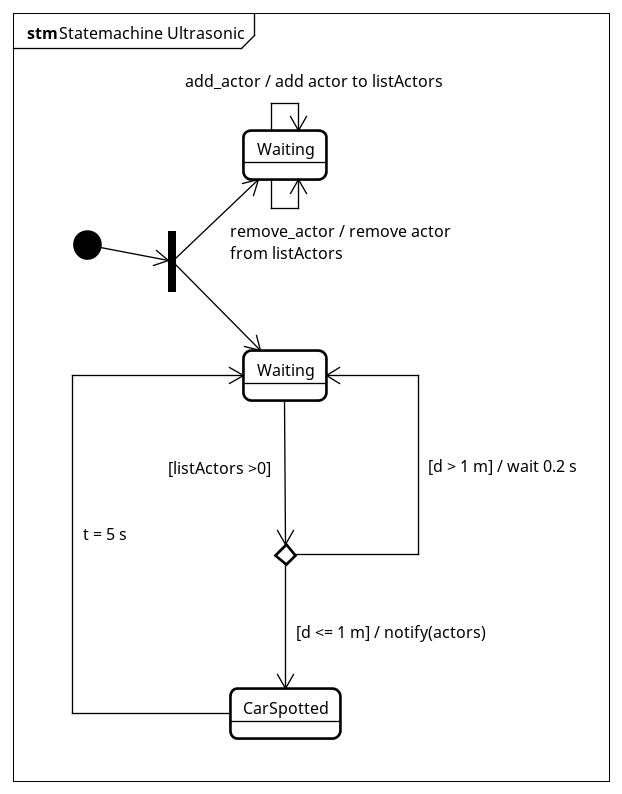
\includegraphics[scale=.75]{figure/Statemachine_Ultrasonic.png}
	\caption{Finished State Machine riguardante la parte di controllo presenza auto \label{FSM CAR}}
\end{figure}
\paragraph{Cambiamento di stato dei lampioni}
Utilizzando il diagramma di sequenza in figura \ref{SD CAR} è stato rappresentato il cambio di stato da parte di due lampioni dal risparmio energetico alla piena potenza dopo la rilevazione di un'auto in transito.
Inizialmente i lampioni si trovano nello stato di risparmio energetico e viene effettuata una misurazione da parte del sensore di prossimità che restituisce la lettura rappresentata da 'd'.
In seguito viene eseguita una seconda lettura e questa volta la distanza rilevata si assume equivalga a meno di un metro, e quindi che sia stata rilevata un'automobile.
Per questo vengono notificati entrambi i lampioni, i quali, dopo un intervallo di tempo calcolato tramite la moltiplicazione tra una costante e il proprio id, passano in modalità piena potenza per permettere all'automobilista di percorrere la strada in sicurezza.
\begin{figure}[tbp]
	\centering
	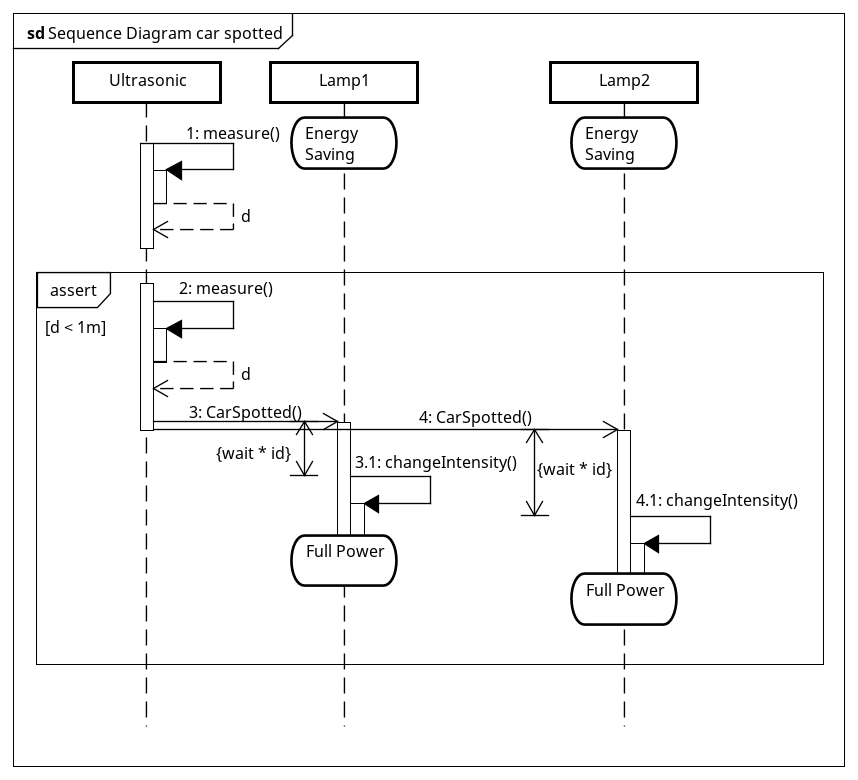
\includegraphics[scale=.59]{figure/Sequence_Diagram_car_spotted.png}
	\caption{Comunicazione tra il sensore ad ultrasuoni e i lampioni rappresentata tramite un Sequence Diagram \label{SD CAR}}
\end{figure}

\subsection{Controllo luminosità ambientale}
Questa parte si occupa di controllare l'intensità luminosa ambientale e di notificare i lampioni in modo che possano accendersi o spegnersi se il valore di luminosità sia maggiore o minore di una certa soglia impostata nelle loro policy.
\paragraph{Architettura}
Per la rappresentazione dell'architettura è stato scelto di utilizzare una Finished State Machine.
In figura \ref{FSM PR} viene mostrato come inizialmente siano generati due thread concorrenti. Come per il caso del controllo della presenza di auto, anche qui un thread è responsabile della gestione della lista dei lampioni da notificare. Il secondo thread invece si occupa di eseguire la lettura dell'intensità luminosa e di notificare ogni lampione presente nella lista.
Il secondo thread parte dallo stato "waiting" ed esegue una lettura se la lista dei lampioni non è vuota. In seguito invia la lettura effettuata a tutti gli elementi della lista e aspetta nello stato "prMeasured" 10 secondi. Infine torna nello stato "waiting".
\begin{figure}[tbp]
	\centering
	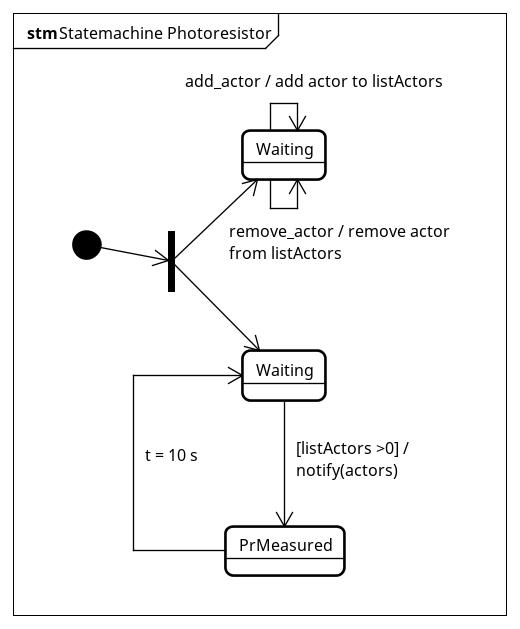
\includegraphics[scale=.8]{figure/Statemachine_Photoresistor.png}
	\caption{Finished State Machine riguardante la lettura della luminosità ambientale \label{FSM PR}}
\end{figure}

\newpage
\subsection{Web Server}
Il web server deve poter comunicare con i Raspberry Pi dislocati sul territorio per poter ottenere e modificare le impostazioni locali di ogni dispositivo.
Per questo scopo il web server si mette in comunicazione con i Raspberry utilizzando le loro interfacce (TODO: si chiamano interfacce?) REST.
\paragraph{Diagramma di sequenza}
Come si può vedere in figura \ref{SD WEB} per la rappresentazione della comunicazione tra il web server e i Raspberry è stato utilizzato un diagramma di sequenza.
Nel primo esempio viene mostrata la richiesta da parte di un utente di ricevere le policy relative al lampione numero 1 da un determinato Raspberry.
Il web server utilizzando un url prestabilito effettua una GET. Il Raspberry ottiene le policy in formato json dal lampione 1 e restituisce tali informazioni al web server che successivamente le mostrerà all'utente.
Il secondo esempio è simile al primo con la differenza che in questo caso l'utente intende effettuare una modifica alla policy on del lampione 1. Quindi il web server questa volta invierà una POST al Raspberry di competenza, il quale notificherà del cambiamento il lampione coinvolto. Infine verrà mostrato all'utente l'esito di tale operazione.
\begin{figure}[tbp]
	\centering
	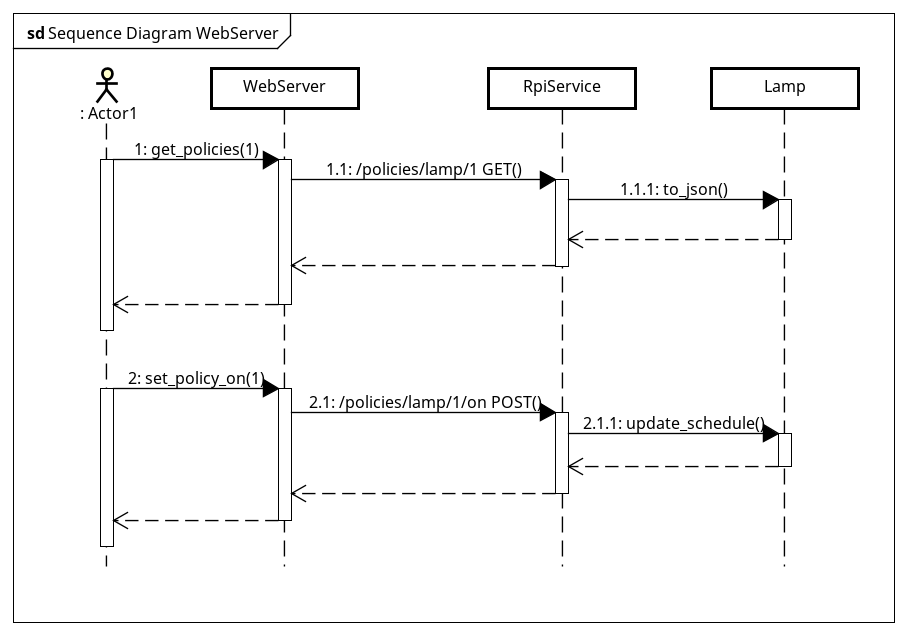
\includegraphics[scale=.55]{figure/Sequence_Diagram_WebServer.png}
	\caption{Sequence diagram per la comunicazione tra web server e Raspberry Pi \label{SD WEB}}
\end{figure}

\newpage
\section{Deployment}
Essendo i vari dispositivi Raspberry necessariamente dislocati sul territorio, si può agire su di essi solo variando il numero di lampioni controllati da ognuno. Per quanto riguarda il lato server, invece, è possibile disaccoppiare i servizi su più server, al fine di migliorare le prestazioni e la ridondanza. Verranno ora descritti i principali metodi di deployment. Sono naturalmente possibili soluzioni intermedie.
\subsection{Centralizzazione totale}
Una soluzione è quella di installare tutti i servizi su un unico server (figura \ref{DD CENT}). Questo minimizza i costi di deployment, ma limita le prestazioni e porta alla costituzione di un pericoloso ``single point of failure''. La riduzione delle prestazioni può non essere un problema nel caso di sistemi di dimensioni ridotte, mentre lo è su sistemi più estesi. La costituzione di un ``single point of failure'', invece, è da tenere bene in considerazione, in quanto un guasto sul server potrebbe causare problemi a tutto il sistema.
\begin{figure}[tbp]
	\centering
	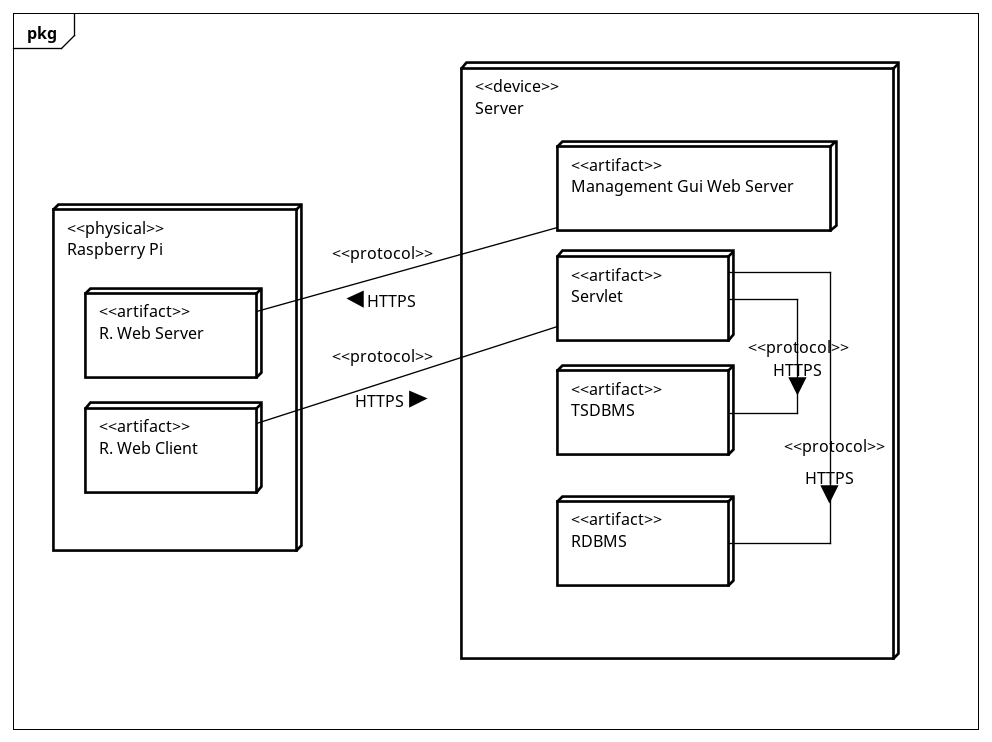
\includegraphics[scale=.5]{figure/Deployment_Diagram_2.png}
	\caption{Diagramma di deployment (server centralizzato) \label{DD CENT}}
\end{figure}
\subsection{Distribuzione}
La soluzione più scalabile e consigliata è quella di installare i vari servizi su server separati (figura \ref{DD DIST}): questo porta ad un forte incremento delle prestazioni, e riduce l'impatto derivante da eventuali guasti.
\begin{figure}[tbp]
	\centering
	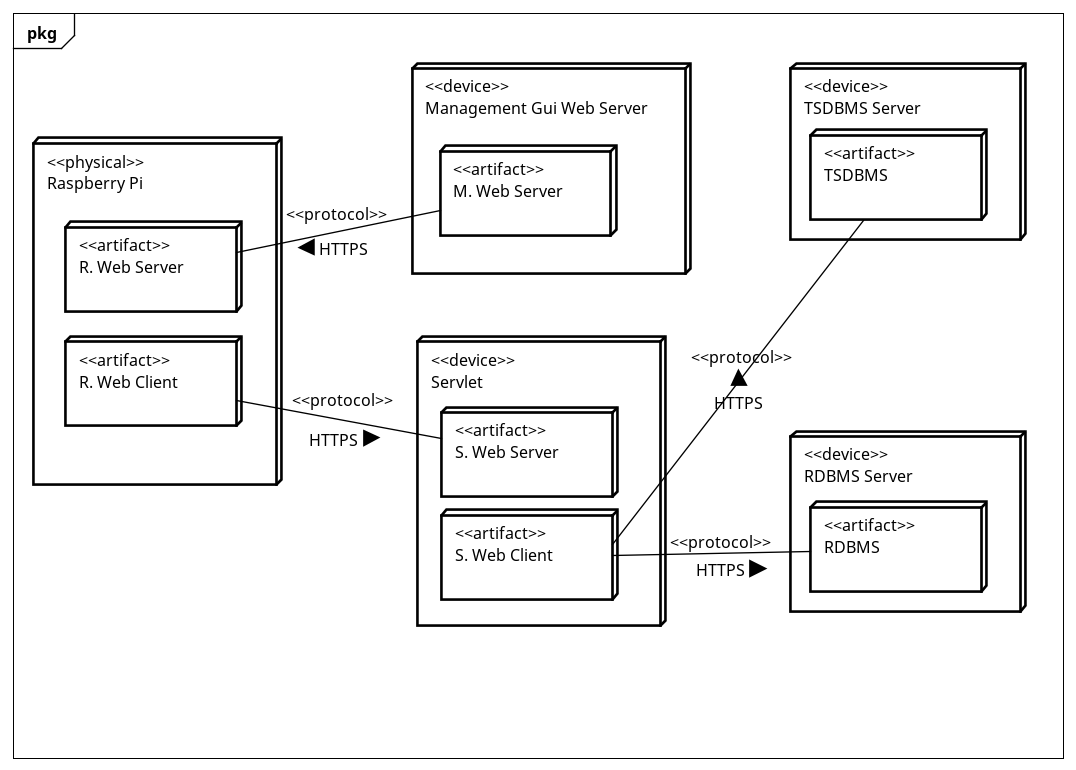
\includegraphics[scale=.45]{figure/Deployment_Diagram_1.png}
	\caption{Diagramma di deployment (server distribuito) \label{DD DIST}}
\end{figure}
\subsection{Layer di smistamento}
Un'ulteriore soluzione prevede di utilizzare un layer di smistamento, installando più istanze della servlet su server diversi. In questo modo il nucleo del traffico non convergerebbe direttamente sul server centrale, ma verrebbe smistato precedentemente, facendo attività di load balancing. Inoltre, in caso di problemi con un'istanza specifica della servlet, solo i Raspberry direttamente collegati ad essa ne risentirebbero.
TODO: immagine


\section{Sicurezza}
TODO